% --- [ Correctness of Implementation ] ----------------------------------------

\subsection{Correctness of Implementation}

% TODO: <note> remove?
% * Test corner cases as they are often the cause of software bugs [x]; such as
%   off-by-one issues and buffer overflow vulnerabilities.
% * Where feasible test all possible inputs; e.g. uint8.

As stated by Edsger W. Dijkstra in 1969, \textit{``testing shows the presence, not the absence of bugs.''} \cite{absence_of_bugs_quote} For this reason, several independent methods were utilized to verify the correctness of the decompilation components and their utility libraries. A lot of thought went into designing test cases which exercise tricky corner cases (e.g. no whitespace between tokens)

% --- [ Subsubsections ] -------------------------------------------------------

% ~~~ [ Test Cases ] ~~~~~~~~~~~~~~~~~~~~~~~~~~~~~~~~~~~~~~~~~~~~~~~~~~~~~~~~~~~

\subsubsection{Test Cases}

% * test in an attempt to break the code, test corner cases, try to imagine how to code may fail.

% TODO: Add
%    - Use the Clang compiler to produce test cases, as it is capable of emitting LLVM IR from C source code. The goal will be to reconstruct the high- level control flow primitives (such as for- loops, if-else statements, etc) of the original C code from the LLVM IR.

% TODO: Add: One risk is that testcases test what you built rather than what was specific in the requirements. TDD solves this.

% TODO: Add: table driven test cases.

foo \ref{fig:iso_test_cases}

\begin{figure}[htbp]
	\begin{center}
		\begin{verbatim}
$ go test -v decomp.org/x/graphs/iso
=== RUN TestCandidates
--- PASS: TestCandidates (0.02s)
=== RUN TestEquationSolveUnique
--- PASS: TestEquationSolveUnique (0.00s)
=== RUN TestEquationIsValid
--- PASS: TestEquationIsValid (0.22s)
=== RUN TestIsomorphism
--- PASS: TestIsomorphism (0.18s)
=== RUN TestSearch
--- PASS: TestSearch (0.20s)
PASS
ok     decomp.org/x/graphs/iso   0.62s
		\end{verbatim}
		\caption{An extract of the test cases used to verify the subgraph isomorphism search library, as visualized by \texttt{go test}.}
		\label{fig:iso_test_cases}
	\end{center}
\end{figure}

% ~~~ [ Code Coverage ] ~~~~~~~~~~~~~~~~~~~~~~~~~~~~~~~~~~~~~~~~~~~~~~~~~~~~~~~~

\subsubsection{Code Coverage}
\label{sec:ver_code_coverage}

Code coverage is a measurement for tracking what parts of the code that gets executed when running test cases. The Go project takes an interesting approach to tracking code coverage, which utilizes the production quality source code analysis and transformation libraries available in Go. Instead of generating platform-dependent assembly which tracks the execution of various branches, Go inject unique tracking statements on each line of the original source code. This approach is platform-independent by design, and may easily be extended to support heat maps which track how often each line gets executed \cite{go_cover}.

As the lexer of any language is a fundamental building block on which other libraries and components depend, the test cases of the LLVM IR lexer aimed for a 100\% code coverage of any code not related to input/output errors (e.g. ``file not found''); as illustrated in figure \ref{fig:lexer_code_coverage}. This rigorous testing uncovered several faulty assumptions in the lexing logic, which were later corrected.

\begin{figure}[htbp]
	\begin{center}
		\begin{verbatim}
$ go test -coverprofile=lexer.out github.com/llir/llvm/asm/lexer
$ go tool cover -func=lexer.out
llvm/asm/lexer/lexer.go:36:    ParseFile      80.0%
llvm/asm/lexer/lexer.go:118:   emit           100.0%
llvm/asm/lexer/lexer.go:139:   next           100.0%
llvm/asm/lexer/lexer.go:158:   accept         100.0%
llvm/asm/lexer/state.go:38:    lexToken       100.0%
llvm/asm/lexer/state.go:131:   lexComment     100.0%
…
llvm/asm/lexer/state.go:364:   lexQuote       100.0%
llvm/asm/lexer/state.go:585:   unescape       100.0%
total:                         (statements)   97.6%
		\end{verbatim}
		\caption{A summary of the code coverage for a selection of the LLVM IR lexer functions, as visualized by the \texttt{cover} tool.}
		\label{fig:lexer_code_coverage}
	\end{center}
\end{figure}

A breif summary of the code coverage for the various software artefacts is presented in figure \ref{tbl:code_coverage_summary}.

\begin{table}[htbp]
	\begin{center}
		\begin{tabular}{|l|l|}
			\hline
			Code coverage & Component \\
			\hline
			97.6\% & LLVM IR lexer \\
			0.0\% & Control flow generation tool \\
			94.8\% & Subgraph isomorphism search library \\
			40.0\% & Control flow analysis tool \\
			0.0\% & Code generation tool \\
			38.0\% & Post-processing tool \\
			\hline
		\end{tabular}
	\end{center}
	\caption{A summary of the code coverage of each component, presented roughly in the same order as they appear in the decompilation pipeline.}
	\label{tbl:code_coverage_summary}
\end{table}

Code coverage heat maps may be used to gain clarity in how often a line gets executed by the test cases. The use of heat maps were invaluable when stress testing the various prototypes of the subgraph isomorphism search algorithm, as they were able to identify several tricky corner cases; such as the ones illustrated in figure \ref{fig:iso_heat_map}

\begin{figure}[htbp]
	\begin{center}
		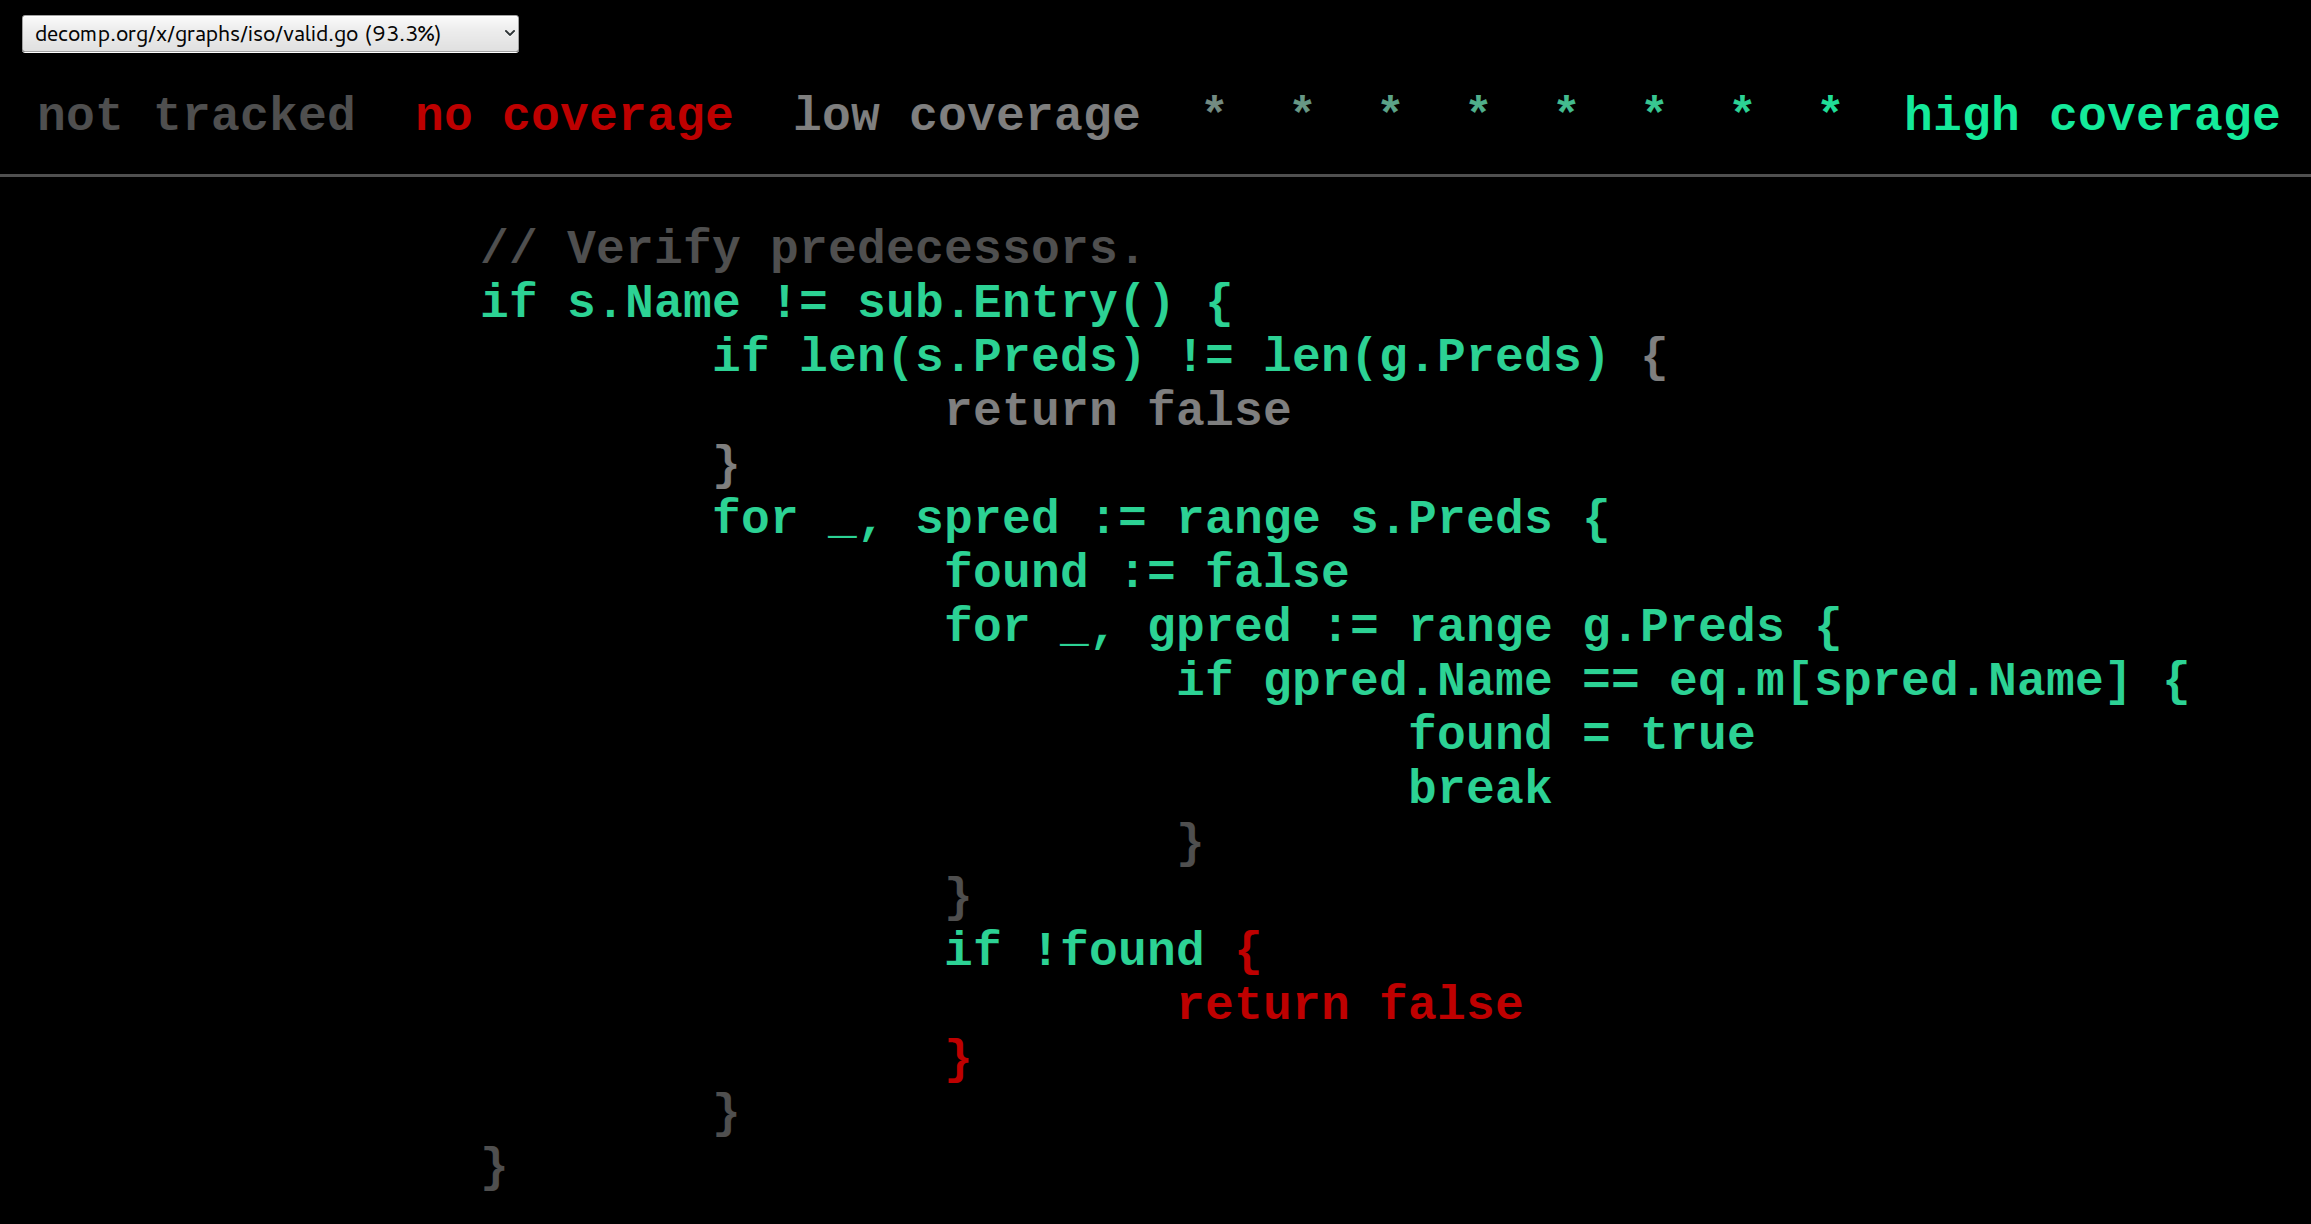
\includegraphics[width=\textwidth]{inc/8_ver/iso_heat_map.png}
		\caption{An extract from the code coverage heat maps of the subgraph isomorphism search algorithm, which has identified two corner cases that may require further validation. The first return statement is seldomly executed (as indicated by the \textit{gray} color), and the second return statement is never executed.}
		\label{fig:iso_heat_map}
	\end{center}
\end{figure}

